% figures/key-types.tex
\documentclass[11pt]{article}
\usepackage[margin=1.5cm]{geometry}
\usepackage{tikz}
\usetikzlibrary{positioning,arrows.meta}
\pagestyle{empty}
\begin{document}
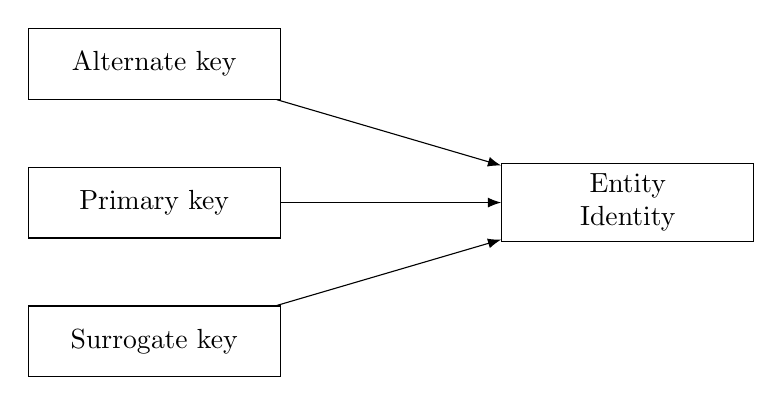
\begin{tikzpicture}[node distance=14mm, >=Latex]
  \node[draw, rectangle, minimum width=3.2cm, minimum height=1cm, align=center] (entity) {Entity\\Identity};
  \node[draw, rectangle, minimum width=3.2cm, minimum height=0.9cm, left=28mm of entity] (pk) {Primary key};
  \node[draw, rectangle, minimum width=3.2cm, minimum height=0.9cm, above left=8mm and 28mm of entity] (ak) {Alternate key};
  \node[draw, rectangle, minimum width=3.2cm, minimum height=0.9cm, below left=8mm and 28mm of entity] (sk) {Surrogate key};

  \draw[->] (pk) -- (entity);
  \draw[->] (ak) -- (entity);
  \draw[->] (sk) -- (entity);
\end{tikzpicture}
\end{document}
